\documentclass{beamer}

\newcommand{\week}{Returns: Measurement}

\title{Financial Market Returns}
\subtitle{Measurement \\ Reference: Bodie et al, Ch 5}
\author{Econ 457}
\date{\week}

% Reference the shared preamble
\input{preamble}

% Set the footer -- change 
\setbeamertemplate{footline}{
  \leavevmode%
  \vspace{2ex}
  \hbox{%
    % Left box: Econ 457
    \begin{beamercolorbox}[wd=.4\paperwidth,ht=2.5ex,dp=1ex,left]{author in head/foot}%
      \hspace{1em}Econ 457
    \end{beamercolorbox}%
    % Middle box: Week
    \begin{beamercolorbox}[wd=.2\paperwidth,ht=2.5ex,dp=1ex,center]{date in head/foot}%
      \centering\week
    \end{beamercolorbox}%
    % Right box: Slide numbers
    \begin{beamercolorbox}[wd=.4\paperwidth,ht=2.5ex,dp=1ex,center]{date in head/foot}%
      \hfill\insertframenumber{} 
    \end{beamercolorbox}%
  }%
  \vskip0pt%
}

\begin{document}

\frame{\titlepage}

\begin{frame}
    \frametitle{Outline}

    \begin{enumerate}
        \item Exponential and Logarithm
        \item Total Returns
        \begin{itemize}
            \item Income
        \end{itemize}
        \item Measurement Issues: 
        \begin{itemize}
            \item Compounding: HPR, EAR, APR, $r_{cc}$
            \item Geometric v. Arithmetic Mean
            \item Log Scale
        \end{itemize}
    \end{enumerate}
\end{frame}

\begin{foundframe}[t]
    \frametitle{1. Exponential and Logarithm}
    \section{Exponential and Logarithm}
    \framesubtitle{Some basic facts}

    Exponential Function:
    $$10^4 = 10 \times 10 \times 10 \times 10$$

    First derivative:
    $$\frac{d(e^x)}{dx} = e^x$$

    Negative Exponents:
    $$a^{-x} = \frac{1}{a^x}$$

    Fractional Exponents:
    $$a^{1/x} = \sqrt[x]{a}$$

\end{foundframe}

\begin{foundframe}[t]
    \frametitle{1. Exponential and Logarithm}
    \framesubtitle{Some basic facts, cont'd}

    Logarithm is the inverse of the exponential function.  $log_{10}()$ is the inverse of $10^x$ and $ln()$ is the inverse of $e^x$
    \vspace{1em}

    First derivative:
    $$\frac{d(ln(x))}{dx} = \frac{1}{x}$$

    Logarithms of expressions with exponents:\\
    $$log(x^a) = a \cdot log(x)$$

    Logarithm of expressions with products:\\
    $$log(x \cdot y) = log(x) + log(y)$$


\end{foundframe}

\begin{foundframe}[t]
    \frametitle{1. Exponential and Logarithm}
    \framesubtitle{Some basic facts, cont'd}

    Two more useful facts about logarithms:
    \begin{enumerate}
    \item  In a log-linear graph the scale of the y-axis is $log(y)$ or $ln(y)$.  
    The slope of the log-linear graph is the average (continuously compounded) growth rate.
    \item Logarithm is a concave function:\\
    $$log((a+b)/2) > (log(a) + log(b))/2$$
    \end{enumerate}

\end{foundframe}


\begin{foundframe}[t]
    \frametitle{1. Exponential and Logarithm}
    \framesubtitle{Some basic facts, cont'd}

    \centering
    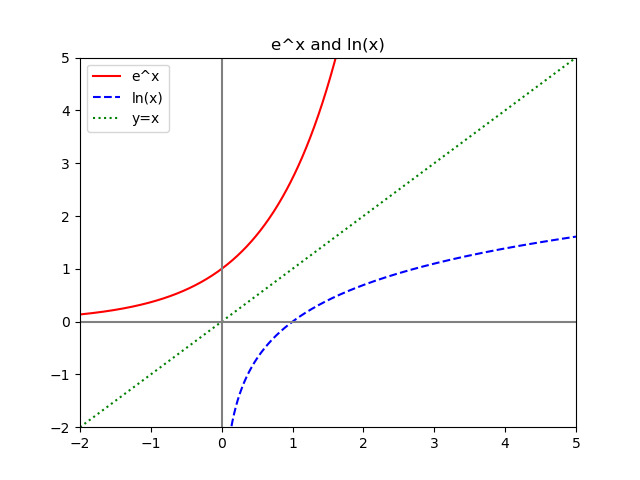
\includegraphics[width=0.8\textwidth]{figures/ch5_1_lnexp.png}

\end{foundframe}


\begin{frame}[t]
    \frametitle{2. Total Returns}
    \section{Total Returns}
    \framesubtitle{Total Return - Definition}

    Total Return: A performance metric that accounts for
    capital gains (i.e. changes in price) and income (e.g. dividends, coupons, etc) 
    paid to the owner of a financial security.\\
    \vspace{1em}   
    Total return is typically expressed as a percentage of the initial price.
    $$
    \text{Total Return} = \frac{\text{Income}}{\text{Initial Price}} + \frac{\text{Change in Price}}{\text{Initial Price}}
    $$
    The first term is sometimes referred to as either the "current yield" or "dividend yield",
     and the second term is referred to as the "capital gain rate."

\end{frame}

\begin{frame}[t]
    \frametitle{2. Income}
    \framesubtitle{Types of Income}

    \begin{table}
        \centering
        \caption{Income Sources by Investment Type}
        \begin{tabular}{lll}
            \toprule
            Investment Type & Income Source & Frequency\\
            \midrule
            Bonds & Coupon payments & Semi-annual (usually) \\
            Stocks & Dividends & Quarterly \\
            ETFs & Distributions & Quarterly/Annual \\
            \bottomrule
        \end{tabular}
    \end{table}
    \vspace{1em}
    ETF distributions are often composed of dividends or coupons of the underlying assets, but occasionally will include capital gains as well.

\end{frame}

\begin{frame}[t]
    \frametitle{2. Income}
    \framesubtitle{Treasury Bond: Note the ``coupons'' at the bottom}
    \centering
    \includegraphics[width=0.5\textwidth]{figures/intro_b_fig3.png}

    \blfootnote{Source: The Joe I. Herbstman Memorial Collection of American Finance}

\end{frame}

\begin{frame}[t]
    \frametitle{2. Income}
    \framesubtitle{Timing of Income}

    Be careful with the timing of income.   
    Often a problem will say "you purchase a stock that just paid a dividend." 
    Do NOT count that dividend in the total return.
    \vspace{1em}

    \centering
    
\includegraphics[width=1\textwidth]{figures/ch5_1_timeline.png}

\end{frame}

\begin{frame}[t]
    \frametitle{2. Income}
    \framesubtitle{Example: AAPL}

    \vspace{-1em}
    \begin{columns}
        \begin{column}{0.48\textwidth}
            \centering
            \begin{table}
            \caption{AAPL Dividends in 2024}
                \begin{tabular}{lr}
                    \toprule
                    date & dividend \\
                    \midrule
                    2024-02-09 & 0.24 \\
                    2024-05-10 & 0.25 \\
                    2024-08-12 & 0.25 \\
                    2024-11-08 & 0.25 \\
                    \bottomrule
                \end{tabular}
            \end{table}
        \end{column}

        \begin{column}{0.48\textwidth}
            \centering
            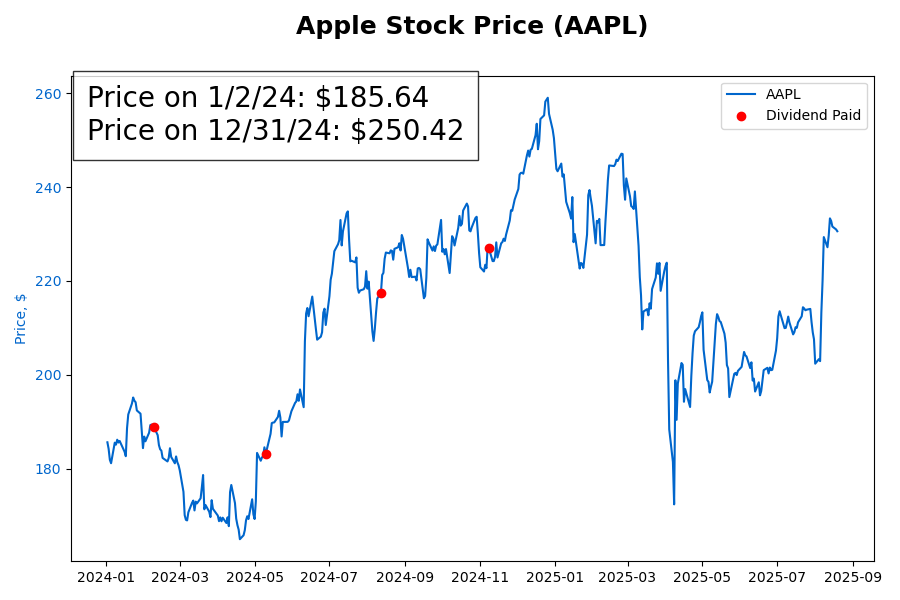
\includegraphics[width=\textwidth]{figures/ch5_1_appl_wincome.png}
        \end{column}
    \end{columns}
    \vspace{1em}

    The price of AAPL was 185.64 on January 2, 2024.   
    The price of AAPL rose to 250.42 on December 31, 2024.  
    What was the Total Return from owning AAPL stock throughout 2024?

    \blfootnote{Data source: Yahoo finance}

\end{frame}

\begin{frame}[t]
    \frametitle{2. Income}
    \framesubtitle{Example: S\&P Total Return}

    \centering
    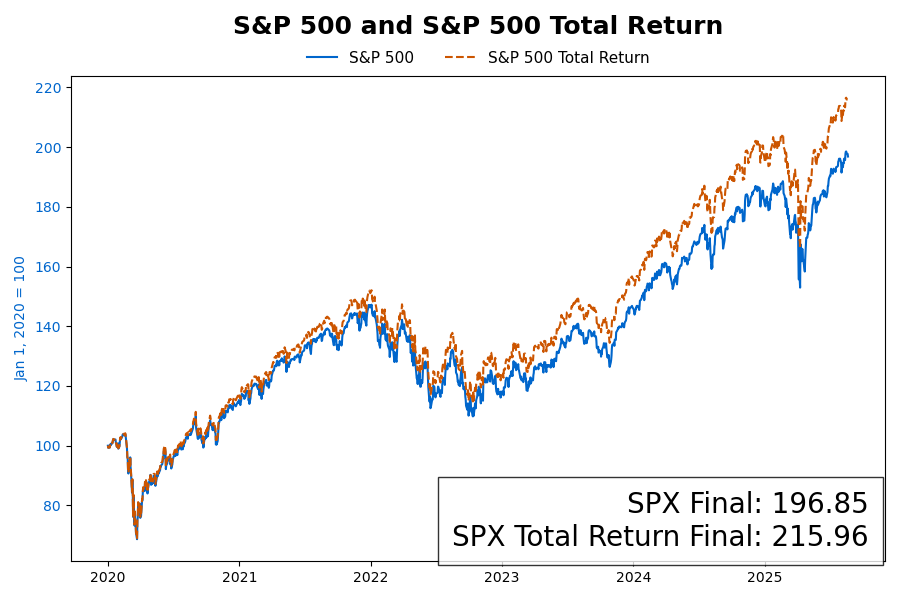
\includegraphics[width=0.8\textwidth]{figures/ch5_1_sp500_tr.png}

    \blfootnote{Data source: Interactive Brokers (SPX and SPXT)}

\end{frame}

\begin{frame}
    \frametitle{3. Measurement Issues}
    \section{Measurement Issues}
    \subsection{HPR}
    \framesubtitle{Holding Period Return}

    Holding Period Return (HPR):\\
    $$\text{HPR} = r(T) = \frac{\text{Price Increase + Income}}{\text{Initial Price}}$$

\end{frame}

\begin{frame}[t]
    \frametitle{3. Measurement Issues}
    \subsection{EAR}
    \framesubtitle{Effective Annual Return}

    The Effective Annual Rate (EAR) expresses the total return as a \textit{rate} of return over a year.   The EAR makes an adjustment for cases when the holding period was not equal to one year\\
    \vspace{1em}

    Effective Annual Rate (EAR)\\
    $$\text{EAR} = (1+\text{HPR})^{1/T} - 1$$\\
    \begin{itemize}
        \item Where T is the length of time the investment was held in years.  
        \item T could be less than one, and could include fractions of years.   For example, a holding period of one and a half years would have $T=1.5$\\
    \end{itemize}

\end{frame}

\begin{frame}[t]
    \frametitle{3. Measurement Issues}
    \subsection{APR}
    \framesubtitle{Annual Percentage Rates}

    The Annual Percentage Rate of Return (APR) is a convention often used for short term instruments.   The rate of return for a single period is equal to $\frac{APR}{n}$, where $n$ is the number of periods in a year. \\
    
    \vspace{1em}
    
    For example, for a credit card with monthly compounding, the monthly rate is equal to the APR divided by twelve.  The APR does not itself account for the effect of compounding, it is only used to determine the size of the monthly payments. 
    
\end{frame}

\begin{frame}[t]
    \frametitle{3. Measurement Issues}
    \framesubtitle{Annual Percentage Rates}

    The relationship between the APR and the EAR is given by:\\
    $$(1 + \text{EAR}) = \left(1+\frac{APR}{n}\right)^n$$\\
    $$\text{APR} = n \times [(1+\text{EAR})^{1/n} - 1]$$

    \begin{itemize}
        \item The APR does not explicitly account for the effects of compounding.   The APR will be lower than the EAR because the EAR \textit{does} account for compounding.\\

    \end{itemize}

\end{frame}




\begin{frame}[t]
    \frametitle{3. Measurement Issues}
    \subsection{$r_{cc}$}
    \framesubtitle{Definition of e}

        The exponential function $e^x$ can be defined as a limit:
    \[
        e^x = \lim_{n \to \infty} \left(1 + \frac{x}{n}\right)^n
    \]
    Notice the similarity to the formula for the APR.\\
    \vspace{1em}
    As $n \to \infty$ the formula for the $APR \to e^{r_{cc}}$, 
    where $r_{cc}$ is the "continuously compounded" rate of return.

\end{frame}    

\begin{frame}[t]
    \frametitle{3. Measurement Issues}
    \framesubtitle{Continuous Compounding}

    Continuously compounded rate of return $(r_{cc})$:
    $$1 + \text{EAR} = exp(r_{cc}) = e^{r_{cc}}$$
    
    \begin{itemize}
        \item If you are given $e^{r_{cc}}$, then with a little rearranging you can find $EAR$: $\text{EAR} = e^{r_{cc}} - 1$
        \item Conversely, if you are given $EAR$ then you can take $ln()$ of both sides to find $r_{cc}$
        \item Note that the $r_{cc}$ will be lower than the EAR because the $r_{cc}$ has more compounding.
    \end{itemize}
    \vspace{1em}

\end{frame}

\begin{practiceframe}
    \frametitle{3. Measurement Issues}
    
    \begin{enumerate}
        \item You purchase a security on January 1st for \$98.  The security produces quarterly income of \$2.  You sell the security after 9 months for \$105.   Calculate the following:
    \begin{itemize}
        \item HPR
        \item EAR
    \end{itemize}
    \item An instrument has a APR of 15\% and makes monthly payments.  Calculate the following:
        \begin{itemize}
        \item Monthly interest rate (in \%)
        \item EAR
        \item $r_{cc}$
    \end{itemize}
    \item An investment has an EAR of 10\% and compounds monthly. Calculate the following:
    \begin{itemize}
        \item APR
        \item $r_{cc}$
        \item The monthly interest rate
    \end{itemize}
    \end{enumerate}
    
\end{practiceframe}

\begin{frame}[t]
    \frametitle{3. Measurement Issues}
    \subsection{Geometric v Arithmetic mean}
    \framesubtitle{Geometric v. Arithmetic Mean}

    For a series of returns, the \textit{arithmetic} average is:
    $$1+ r_{ave} = \frac{1}{T}\times\sum_{i=1}^{T}(1 + r_i)$$

    The \textit{geometric} average is:
    $$1+ r_{geo-ave} = \sqrt[T]{\prod_{i=1}^{T} (1 + r_i)}$$

\end{frame}

\begin{frame}[t]
    \frametitle{3. Measurement Issues}
    \framesubtitle{Geometric v. Arithmetic Mean}

    The arithmetic average is \underline{greater than or equal to} the geometric average.  Equality occurs when all of the observations are the same.\\
    \vspace{1em}
    You can show this using the fact that the $ln()$ function is concave (next slide).\\
    
    \vspace{1em}
    The difference between the arithmetic and geometric averages is increasing in the variance of the return series.

\end{frame}

\begin{frame}[t]
    \frametitle{3. Measurement Issues}
    \framesubtitle{Geometric v. Arithmetic Mean}

    \footnotesize
    Showing that the Geometric Mean $<$ the Arithmetic Mean.  Let $r_i$ be the return, and $x_i = 1+r_i$.
    \begin{align}
        \text{Geometric Mean} = \sqrt[T]{\prod_{i=1}^{T} x_i}\\
        \ln(\text{Geometric Mean}) = \frac{1}{T} \sum_{i=1}^{T} \ln(x_i)\\
        < \ln\left(\frac{1}{T} \sum_{i=1}^{T} (x_i)\right)\\
        < \ln(\text{Arithmetic Mean})\\
        \implies \text{Geometric Mean} < \text{Arithmetic Mean}
    \end{align}
    Where (2) applies properties of $ln()$, (3) is because $ln()$ is a concave function 
    (Jensen's inequality), and (4) is because $ln()$ is monotonically increasing.

\end{frame}

\begin{frame}[t]
    \frametitle{3. Measurement Issues}
    \framesubtitle{Geometric v. Arithmetic Mean}

    \footnotesize

    Alternative proof that the Geometric Mean $<$ the Arithmetic Mean in the case of only two observations
    \vspace{1em}
    
    Definitions: Geometric Mean: $\sqrt{XY}$, Arithmetic Mean $\frac{X+Y}{2}$
    
    \vspace{1em}
    
    Show $$\frac{X+Y}{2} \geq \sqrt{XY}$$
    \begin{align*}
        \left(\frac{X+Y}{2}\right)^2 \geq XY \\
         X - 2\sqrt{XY} + Y \geq 0 \\
        \text{let } a = \sqrt{X}, b = \sqrt{Y} \\
        a^2 - 2ab + b^2 \geq 0 \\
        (a - b)^2 \geq 0 \\
    \end{align*}

\end{frame}

\begin{frame}[t]
    \frametitle{3. Measurement Issues}
    \framesubtitle{Geometric v. Arithmetic Mean, Example}

    Stock ABC doesn't pay dividends.   In year 1 the price of ABC declines by 20\%.   
    In year 2 the price rebounds by 20\%.\\ 
    \vspace{1em} 
    What is the arithmetic average of the annual returns?   What is the geometric average?
    \vspace{1em}
    Which measure is more appropriate?

\end{frame}

\begin{practiceframe}[t]
    \frametitle{3. Measurement Issues}
    \framesubtitle{Geometric v. Arithmetic Mean}

    We can use the same concept to compute the distrubtion for a longer time period.

  \begin{enumerate}
  \setcounter{enumi}{1}
    \item You invest \$1 million at the beginning of 2028 in a stock-index fund. 
    If the rate of return in 2028 is -40\%, what rate of return in 2029 will be necessary for your portfolio to recover to its original value.
  \end{enumerate}

\end{practiceframe}



\begin{frame}[t]
    \frametitle{3. Measurement Issues}
    \framesubtitle{Arithmetic v. Geometric Mean}
    
    \vspace{-1em}
    \scriptsize
    \begin{table}
    \caption{S\&P 500 Total Returns by Decade, (\% Annualized)}
    \begin{tabular}{lrrr}
    \toprule
    Decade & Arithmetic Return & Geometric Mean & Standard Deviation \\
    \midrule
    1870s & 8.11 & 7.46 & 10.86 \\
    1880s & 6.29 & 5.83 & 9.62 \\
    1890s & 6.24 & 5.55 & 11.84 \\
    1900s & 10.62 & 9.82 & 12.70 \\
    1910s & 4.99 & 4.44 & 10.51 \\
    1920s & 15.46 & 14.25 & 15.08 \\
    1930s & 4.39 & 0.03 & 30.63 \\
    1940s & 9.47 & 8.58 & 13.23 \\
    1950s & 18.24 & 17.74 & 10.08 \\
    1960s & 8.05 & 7.51 & 10.31 \\
    1970s & 6.56 & 5.69 & 13.23 \\
    1980s & 16.88 & 16.04 & 12.98 \\
    1990s & 17.19 & 16.66 & 10.45 \\
    2000s & 0.38 & -0.73 & 14.68 \\
    2010s & 13.02 & 12.56 & 9.55 \\
    2020s & 13.72 & 12.11 & 14.15 \\
    \bottomrule
    \end{tabular}
    \end{table}

    \blfootnote{Data Source: Robert Shiller, Ken French.  Monthly data annualized.}

\end{frame}

\begin{frame}[t]
    \frametitle{3. Measurement Issues}
    \subsection{Log Scale}
    \framesubtitle{Log scale}

    In a log-linear graph, $ln(y)$ is plotted against time.  
    The slope is the average continuously compounded growth rate per unit of time.

    \begin{columns}
        \begin{column}{0.55\textwidth}
            \centering
            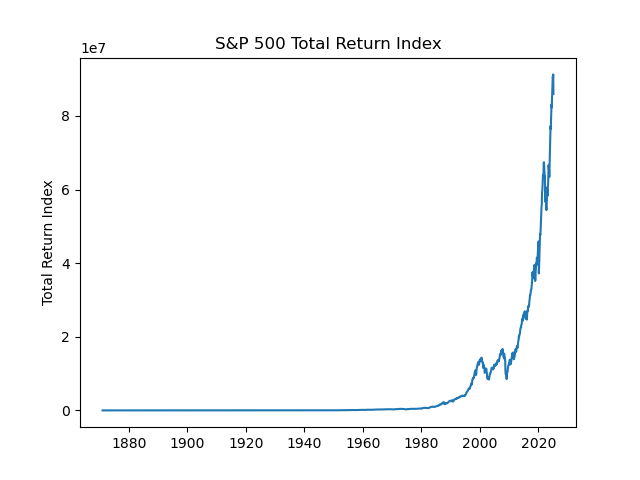
\includegraphics[width=\textwidth]{figures/ch5_1_sp500.png}
        \end{column}
        \begin{column}{0.55\textwidth}
            \centering
            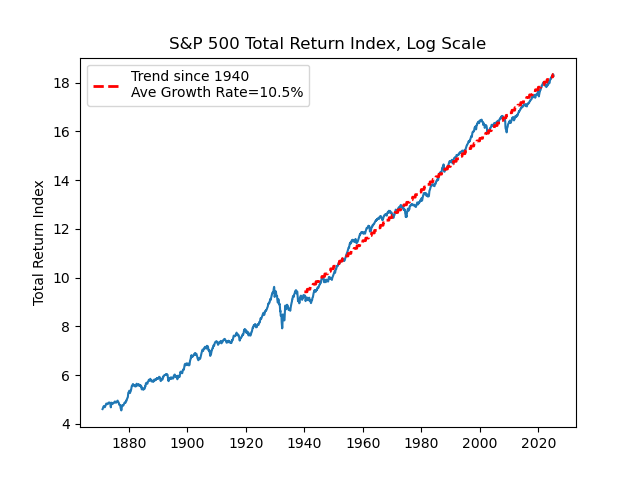
\includegraphics[width=\textwidth]{figures/ch5_1_sp500_logscale.png}
        \end{column}
    \end{columns}

    \blfootnote{\raggedright Data Source: Robert Shiller, www.shillerdata.com}

\end{frame}

\begin{frame}[t]
    \frametitle{3. Measurement Issues}
    \framesubtitle{Things to pay attention to}

    \begin{itemize}
        \item Income
        \item Frequency of compounding
        \item Relationship between EAR and APR.
        \item Relationship between EAR and $r_{cc}$
        \item When are APR and $r_{cc}$ similar?
        \item Geometric or Arithmetic mean?
        \item For longer time series, better to visualize in ln(y)?
    \end{itemize}
    
    \blfootnote{What is the correct treatment of income?  Does it get compounded or not?  It depends on the context.  It's easy to reinvest income from an ETF, it may be harder in a privately held stock.}

\end{frame}

\begin{practiceframe}[t]
  \frametitle{Review: HPR, EAR, APR and $r_{cc}$}
  \framesubtitle{}

  \begin{itemize}
    \item Holding Period Return (HPR)
    $$\frac{\text{Price Change} + \text{Income}}{\text{Initial Price}}$$
    \item Effective Annual Rate (EAR)
    $$(1 + EAR)^T = 1 + HPR$$
    \item Annual Percentage Rate (APR)
    $$1+EAR = \left(1 + \frac{APR}{n}\right)^n$$
    \item Continuously Compounded Rate of Return ($r_{cc}$)
    $$1+EAR = e^{r_{cc}}$$
  \end{itemize}

\end{practiceframe}

\end{document}
